\documentclass[12pt]{article}
 
\usepackage[margin=.75in]{geometry} 
\usepackage{amsmath,amsthm,amssymb}
\usepackage{bm}
\usepackage{enumitem}
\usepackage{color}
\usepackage{graphicx}
\usepackage{verbatim}
\setenumerate{listparindent=\parindent}
\definecolor{gray}{gray}{0.6}

\setenumerate{listparindent=\parindent}
 
\newcommand{\N}{\mathbb{N}}
\newcommand{\Z}{\mathbb{Z}}
\newcommand{\E}{\mathbb{E}}
\DeclareMathOperator*{\Cov}{Cov}
\DeclareMathOperator*{\Col}{Col}
 
\usepackage{listings}
\lstset{
language=R,
basicstyle=\scriptsize\ttfamily,
commentstyle=\ttfamily\color{gray},
%numbers=left,
numberstyle=\ttfamily\color{gray}\footnotesize,
stepnumber=1,
numbersep=5pt,
backgroundcolor=\color{white},
showspaces=false,
showstringspaces=false,
showtabs=false,
frame=single,
tabsize=2,
captionpos=b,
breaklines=true,
breakatwhitespace=false,
%title=\lstname,
escapeinside={},
keywordstyle={},
morekeywords={}
} 

\usepackage{fancyhdr} % Required for custom headers 
%\usepackage{lastpage} % Required to determine the last page for the footer

\pagestyle{fancy}
\lhead{Stat 151A (HW4)}
\chead{Michael Knopf (24457981)}
\rhead{April $13^\text{th}$, 2015}
\lfoot{}
\cfoot{}
\rfoot{}
%\rfoot{Page\ \thepage\ of\ \pageref{LastPage}}
\renewcommand\headrulewidth{0.4pt}
%\renewcommand\footrulewidth{0.4pt}


\begin{document}

\begin{enumerate}[leftmargin=0cm,itemindent=.5cm,labelwidth=\itemindent,labelsep=0cm,align=left]

\item Consider the bodyfat dataset and consider fitting a linear model for the response variable BODYFAT in terms of the explanatory variables AGE, WEIGHT, HEIGHT, ADIPOSITY, NECK, CHEST, ABDOMEN, HIP, THIGH, KNEE, ANKLE, BICEPS, FOREARM, and WRIST.
\begin{enumerate}
\item \ Using each of the following methods, perform variable selection to select a subset of the explanatory variables for modeling the response:
\begin{enumerate}
\item \ Backward elimination using the individual $p$-values
\item \ Forward selection using $p$-values
\item \ Adjusted $R^2$
\item \ AIC
\item \ BIC
\item \ Mallow's $C_p$
\end{enumerate}
\end{enumerate}





\begin{proof}[Solution]
\ Given below are functions I have written which return the model selected by each of these methods.  The adjusted $R^2$ and Mallow's $C_p$ functions use a backward elimination method to select the best model according to these criteria.
\lstinputlisting{./bodyfat.R}
The summaries of each model are given below.  As expected, the AIC method gave the same results as Mallows' CP, and the BIC method returned a model with less variables than the AIC method.
\lstinputlisting{./select.R}

\end{proof}







\begin{enumerate}
\setcounter{enumii}{1}
\item \ Let $M_1, \dots , M_6$ denote the six models selected by each of the six variable selection methods of the previous part.  Select one of these models by cross-validation.
\end{enumerate}


\begin{proof}[Solution]

\ Of the 6 models resulting from the methods in part (a), 5 were the same.  The only model that differed from the others was that obtained using the BIC criterion.  These two models are
\begin{align*}
\text{BODYFAT} &= \text{AGE + WEIGHT + NECK + ABDOMEN + HIP}\\ &\text{\ + THIGH + FOREARM + WRIST}
\\
\text{BODYFAT} &= \text{WEIGHT + ABDOMEN + FOREARM + WRIST}
\end{align*}
where the second model comes from the BIC method and the first is from the other five methods.  The GCV values for these models are 4092.841 and 4152.815, respectively.  This suggests that the first model is better.  I have also written a script, shown below, that simulates general cross-validation.  This was mainly out of curiosity, to check how muc the results would differ from those obtained using GCV.  This method gave the same answer, that the first model is better.

Pure cross-validation suggests that the first model is better, so I will choose this model for the next part.  However, the scores of the two models are very similar, and in practice it might be useful to choose the smaller model, instead.

\lstinputlisting{./cross2.R}






\begin{comment}
\ Below is a script I have written to perform the cross-validation.  I broke the data into 6 equally sized subsets.  It is possible, though unlikely, that one of the sets (say the $k$th) contains many outliers in the Bodyfat category.  This would cause the $k$th model to look like it is not performing well.  To correct for this, I cycled the models so that each model used each training-test pair exactly once, then summed the resulting errors.

So I have used a statistic that is the sum over all 6 partitions of the sum of the squared predicted errors for the $i$th model.  The results are tabulated below.

\begin{center}
\begin{tabular}{|c|c|c|c|c|c|}
\hline 
$M_1$ & $M_2$ & $M_3$ & $M_4$ & $M_5$ & $M_6$ \\ 
\hline
$4435.071$ & $4056.559$ & $3604.224$ & $3980.025$ & $4168.684$ & $4316.852$ \\
\hline 
\end{tabular} 
\end{center}
It appears that the 3rd model is the most effective.  This model was obtained using the adjusted $R^2$ method of variable selection.

\lstinputlisting{./cross.R}
\end{comment}
\end{proof}



\begin{enumerate}
\setcounter{enumii}{2}
\item \ Let $M$ be the model selected in the previous part.  Fit the model to the data.  Perform regression diagnostics.  Comment on the validity of the assumptions of the linear model.  Identify influential observations and outliers.  Delete them if necessary and re-fit the model.
\end{enumerate}



\begin{proof}[Solution]
\ The chosen model is
$$
\text{BODYFAT} = \text{AGE + WEIGHT + NECK + ABDOMEN + HIP + THIGH + FOREARM + WRIST.}
$$
In the script below, I fit the model to the data and performed regression diagnostics.  The left plot below, as well as the 14 plots below it, show evidence for constant variance across the fitted values as well as across each explanatory variable.  The right plot below shows supports the assumption of the normality of the errors.  I have also provided the code used to produce these plots and determine any other observations about the model and the data.

Testing for outliers, using the Bonferroni correction, does not yield any outliers at the $.05$ significance level.  Observations 39 and 224 are influential observations, however.  I have given the summary for the model where these observations have been excluded.  I would use this model rather than the original.

On the last homework, 39 was considered an outlier according to the Bonferroni correction at the $.05$ significance level.  The reason it is not an outlier in this model is that the design matrix has changed, thus its leverage and residual are different.  Perhaps the categories in which it was most different from the other observations are not being used in this model.

Overall, the model appears strong.  The assumption that the errors are normal with constant variance is not contradicted by this evidence.
\begin{figure}[ht!]
\centering
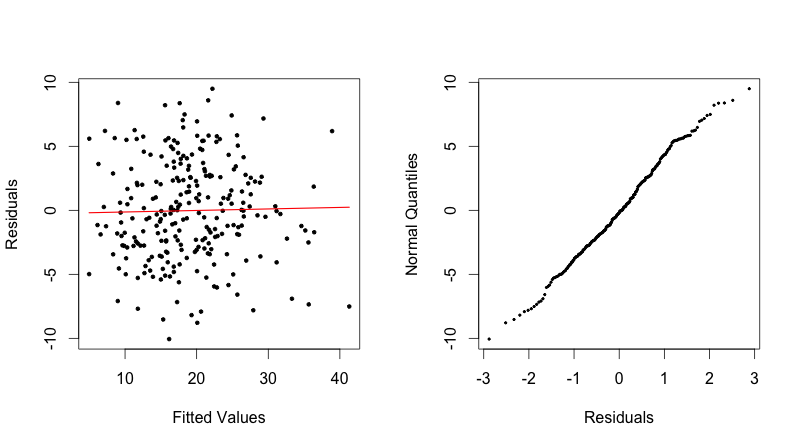
\includegraphics[width=160mm]{fitresnormqq.png}
\end{figure}

\begin{figure}[ht!]
\centering
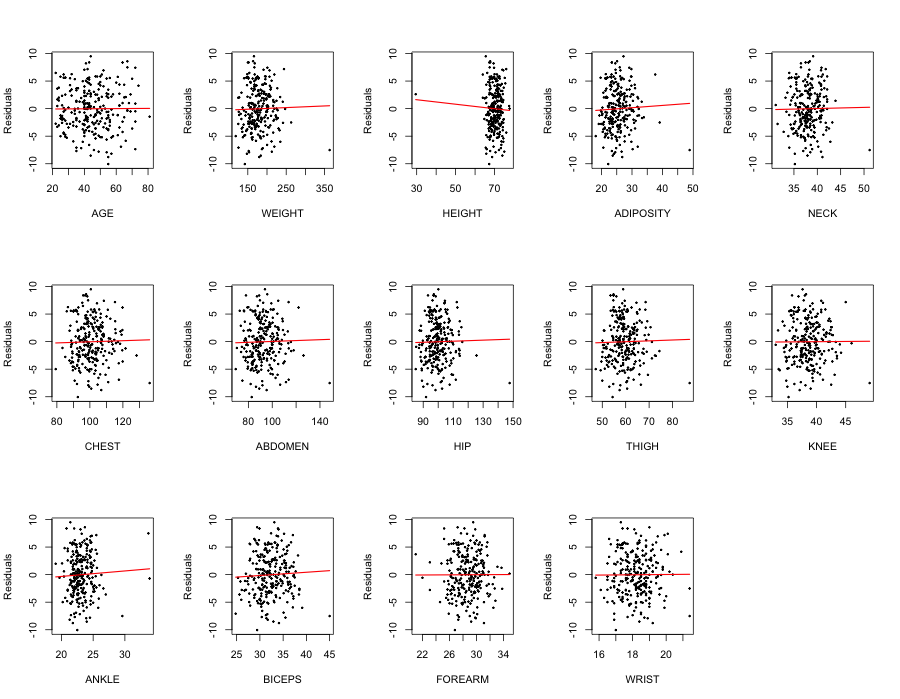
\includegraphics[width=180mm]{manyplots.png}
\end{figure}

\begin{figure}[ht!]
\centering
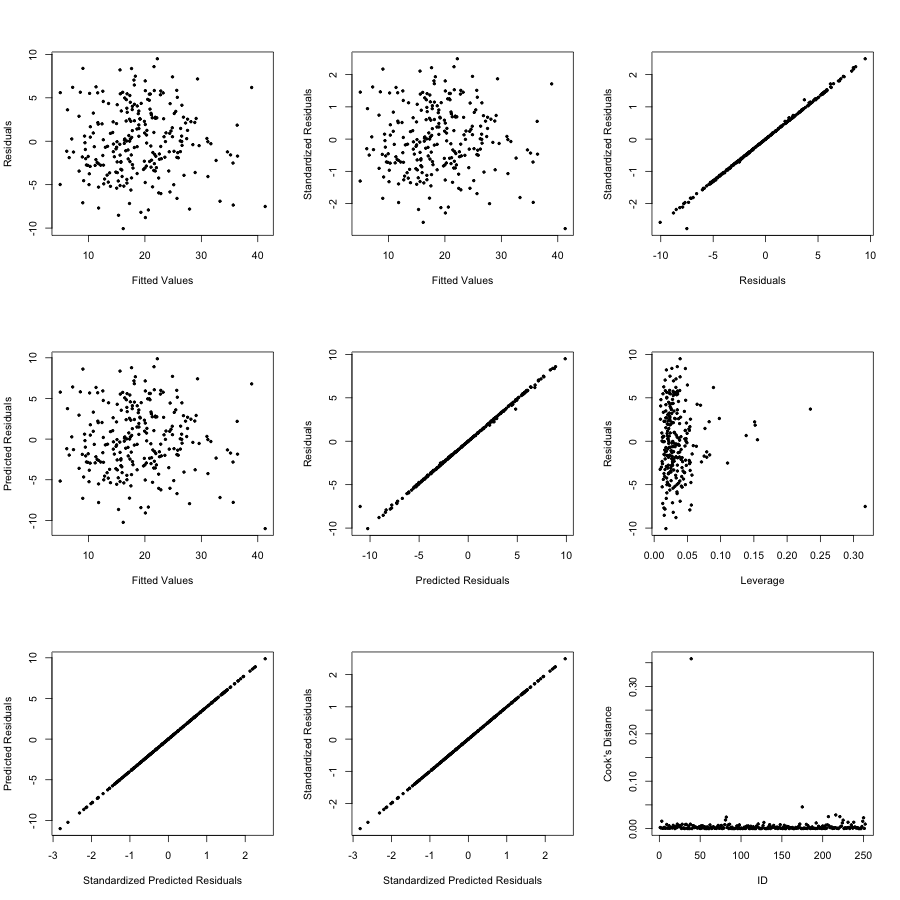
\includegraphics[width=180mm]{outlierplots.png}
\end{figure}

\ \lstinputlisting{./themodel.R}
This is the summary for the model obtained by removing the $39$th and $224$th observations:
\ \lstinputlisting{./newmodel.R}
\end{proof}



\end{enumerate}
\end{document}

















